\documentclass{beamer}

\mode<presentation>
{
  \usetheme{Warsaw}
  \definecolor{links}{HTML}{2A1B81}
  \hypersetup{colorlinks,linkcolor=,urlcolor=links}
  %\usetheme{Frankfurt}
  \usecolortheme{seagull}
  % or ...
  \setbeamercovered{transparent}
  % or whatever (possibly just delete it)
}

\usepackage[english]{babel}
\usepackage[utf8]{inputenc}
\usepackage{times}
\usepackage[T1]{fontenc}
\usepackage{fancyvrb}
\usepackage{listings}
\usepackage{graphicx}
\usepackage{attachfile}
\usepackage{ifthen}

\newboolean{localPieces} %Declaration, defaults to false
\setboolean{localPieces}{false} %Assignment

\title[My Way] % (optional, use only with long paper titles)
{My Way}

\author[Gogins] % (optional, use only with lots of authors)
{Michael Gogins \\ \url{http://michaelgogins.tumblr.com} }
% - Give the names in the same order as the appear in the paper.
% - Use the \inst{?} command only if the authors have different
%   affiliation.

\institute[Irreducible Productions] % (optional, but mostly needed)
{
  Irreducible Productions\\
  New York
}
% - Use the \inst command only if there are several affiliations.
% - Keep it simple, no one is interested in your street address.

\date[6 March 2017] % (optional, should be abbreviation of conference name)
{6 March 2017}
% - Either use conference name or its abbreviation.
% - Not really informative to the audience, more for people (including
%   yourself) who are reading the slides online

\subject{Computer Music}
\expandafter\def\expandafter\insertshorttitle\expandafter{%
    \insertshorttitle\hfill%
    \insertframenumber\,/\,\inserttotalframenumber}
% This is only inserted into the PDF information catalog. Can be left
% out. 
\begin{document}
\lstset{basicstyle=\ttfamily\tiny,commentstyle=\ttfamily\tiny,tabsize=2,breaklines,fontadjust=true,keepspaces=false,fancyvrb=true,showstringspaces=false,moredelim=[is][\textbf]{\\emph\{}{\}}}

\begin{frame}
  \titlepage
\end{frame}

\begin{frame}{Outline}
	I talk about my way of doing algorithmic composition. Many references and examples herein are by hyperlink to the World Wide Web. Most of my pieces are made using \href{http://csound.github.io/}{Csound}. Note: Some track titles got reversed with CDBaby.
  \tableofcontents
  % You might wish to add the option [pausesections]
\end{frame}

\section{My Goals}

\begin{frame}{Motivation}
	\begin{itemize}
		\item
			I've loved classical music since childhood.
		\item
			I made up music in my head, and sometimes I wanted to compose, but I was afraid I had no talent --- and music theory seemed \emph{very} daunting! 
		\item
			A \href{http://labs.la.utexas.edu/gilden/files/2016/04/Gardner-WhiteBrownFractalMusic.pdf}{1978 Martin Gardner column} showed me the Peano snowflake curve, and it occurred to me the horizontal lines could be punched as an interesting piano roll. 
		\item
			When personal computers appeared in the 1980s, I started experimenting with algorithmic composition.
		\item
			But using fractals created problems that dragged me right back into music theory\dots
	\end{itemize}
\end{frame}

\begin{frame}{Peano Snowflake}
	\begin{center}
        \ifthenelse{\boolean{localPieces}}
            {\href{file:///D:/Dropbox/Michael Gogins/Garden of Algorithms/04-Bending Arches.wav}{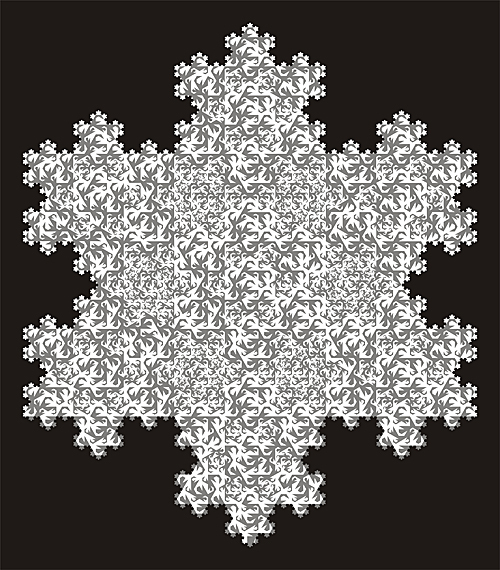
\includegraphics[scale=1.375]{peano_snowflake}}}
            {\href{https://www.youtube.com/watch?v=eJ_d_3wV6i0}{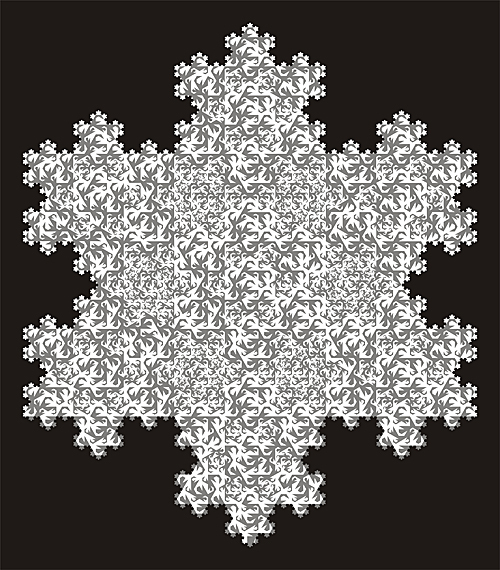
\includegraphics[scale=1.375]{peano_snowflake}}}
	\end{center}
\end{frame}

\begin{frame}{What Is Computer Music?}
	There are many definitions of computer music.
	The most obvious is, ``Computer music is music that is made with a computer, just like piano music is music that is played on the piano.'' But that is not really a good definition, because computers today are used to record, mix, master, publish, and listen to classical music, rock music, jazz, and every other kind of music. Perhaps a better definition is, ``Computer music is music that can \emph{only} be made with a computer.'' In other words, it is music that is \emph{idiomatic} to the computer. But what does that mean?
\end{frame}

\begin{frame}{What Is a Computer Anyway?}
	\begin{itemize}
		\item
			An algorithm is just a procedure that can be carried out step by step to produce a result, without needing to know what the steps \emph{mean}. This is the technical definition. A cookie recipe is an algorithm, so is long division.
		\item
			For any single algorithm, a machine can be built to execute it. Such a machine is called a Turing machine, or \textit{computer}. The idea is basic in logic, mathematics, even physics.
		\item
			A single Turing machine can be built to execute an algorithm that can simulate any and all other Turing machines. Such a machine is called a universal Turing machine, or \textit{programmable computer}.
		\item
			You yourself, a laptop computer, or a smartphone are all physical realizations of universal Turing machines.
		\item
			But a computer can execute algorithms literally \emph{billions of times faster} than you can.
	\end{itemize}
\end{frame}

\begin{frame}{The Musical Idioms of the Computer}
    Since human beings can also compute, the idioms of the computer build upon its blinding speed:
    \begin{itemize}
    	\item 
	    	\textbf{Analysis/Resynthesis} Computers can analyze digital audio, morph it or cross-synthesize it, resynthesize it, and combine it into collages --- in ways that would simply be impossible by hand. Although this is actually the most common kind of computer music, I don't usually do this.
	    \item
	     	\textbf{Algorithmic Composition} Computers can generate musical materials or scores in ways that would just take too long to do by hand. 
	     	\begin{itemize}
	     		\item
		     		\textit{Corpus-based} The computer uses a database of existing materials to generate music by variation and recombination, even using machine learning.
		     	\item
			     	\textit{Mathematics-based} The computer uses fractals or other mathematical procedures to generate scores. This is what I usually do.
	     	\end{itemize}
    \end{itemize}
\end{frame}

\begin{frame}{Why Do Algorithmic Composition?}
	\begin{itemize}
		\item
			Algorithmic composition is the use of algorithms to compose music.
		\item
			But why bother? We already know how to compose.
		\item
			Because it's usually impossible to predict in detail what algorithms will do until you watch them run.
		\item
			Mathematicians call this \emph{computational irreducibility}.
		\item
			Here's a simple example: Tell me what the 1st iteration of $y \Leftarrow \frac{1}{4} \: 0.9384932 \: y \: (1 -y)$ is. The 1,000th iteration.
		\item 
			Therefore, you can use algorithms to create and control things you can't imagine. 
		\item
			Therefore, \emph{algorithms can amplify the imagination.}
	\end{itemize}
\end{frame}


\begin{frame}{Computational Irreducibility}
	\begin{itemize}
		\item
		    Computational irreducibility is what generates the stunning beauty of Nature: branchings, flows, clouds.
		  \item
			Computational irreducibility arises from the iteration of nonlinear operations; in my little example, the nonlinearity comes from squaring $y$.
		  \item
		    Using irreducibility to generate art, whether representational or abstract, deeply illuminates Aristotle's thesis that art is the imitation of Nature.
		 \item 
			Another excellent example of irreducibility is \href{https://www.shadertoy.com/view/MtyGWV}{Conway's Game of Life}, a 2 dimensional cellular automaton: each iteration, each cell lives if exactly 3 of its nearest neighbors is alive, and otherwise dies.
	\end{itemize}
\end{frame}

\begin{frame}{Universal Computer/Constructor in Life}
	\begin{center}
		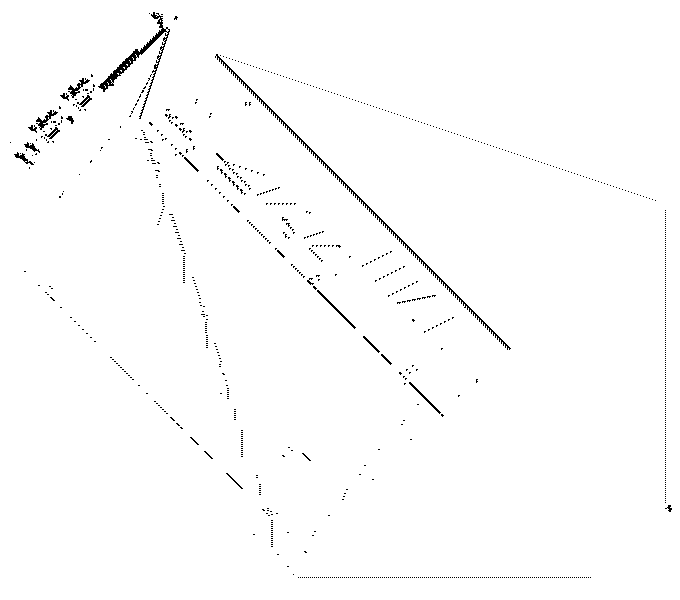
\includegraphics[scale=.3334]{calcyman}
	\end{center}
\end{frame}

\section{My Approach}

\begin{frame}[allowframebreaks]
    \frametitle<presentation>{Algorithms I've Used}
  	\begin{itemize}
  		\item
			I started with chaotic dynamical systems, e.g. \ifthenelse{\boolean{localPieces}}{\href{file:///D:/Dropbox/Michael Gogins/Garden of Algorithms/11-Piano Fall.wav}{\textit{\textbf{Triptych}}}}{\href{https://www.youtube.com/watch?v=eKbqJXb5ZKc}{\textit{\textbf{Triptych}}}}, 2004, chaos mapped onto predetermined chords.     
  		\item
    		1-dimensional cellular automata (rule 110 is also proved capable of universal computation).
  		\item
			Then I played with Mandelbrot sets and Julia sets, and discovered a Mandelbrot-like set for music \cite{G1991}.
 		\item
			Iterated function systems, e.g. \ifthenelse{\boolean{localPieces}}{\href{file:///D:/Dropbox/Michael Gogins/Garden of Algorithms/06-970104e.wav}{\textit{\textbf{Chaotic Squares}}}}{\href{https://www.youtube.com/watch?v=ZTO_8l0FGbU}{\textit{\textbf{Chaotic Squares}}}}, 1991, IFS mapped onto pitch $\times$ time. 
  		\item
			Lindenmayer systems, e.g. \ifthenelse{\boolean{localPieces}}{\href{file:///D:/Dropbox/Michael Gogins/Garden of Algorithms/12-Three Trees.wav}{\textit{\textbf{Cloud Strata}}}}{\href{https://www.youtube.com/watch?v=gjl99B-6el8&list=PLYQnJFl5fDAKoyqwk911PahBnSTar3fb5&index=12}{\textit{\textbf{Cloud Strata}}}}, 1991, 0-L system mapped onto pitch $\times$ time.
  		\item
			I worked with image generating software, and translated images to scores, e.g.  \ifthenelse{\boolean{localPieces}}{\href{file:///D:/IHP100/_ea_/Gogins, Michael/Gogins, Michael -- Semblance/f--2002-01-28--17-37-42.042.mml.9632.1.mp3}{\textit{\textbf{06-f--2002-01-28--17-37-42.042.mml.9632.1}}}}{\href{https://www.youtube.com/watch?v=2nsFJfvEYus}{\textit{\textbf{06-f--2002-01-28--17-37-42.042.mml.9632.1}}}}
 		\item
			I used software like \href{http://kandid.sourceforge.net/gal_favorites_1.html}{Kandid} and \href{http://www.apophysis.org/}{Apophysis} to \textit{evolve} pieces, e.g. \ifthenelse{\boolean{localPieces}}{\href{file:///D:/msys64/home/restore/michael.gogins.studio/music/published/Michael Gogins -- Sound Fractals -- Track 1 -- Sound Fractals.master.wav}{\textit{\textbf{Sound  Fractals}}}}{\href{https://www.youtube.com/watch?v=WuntpYyubfc}{\textit{\textbf{Sound Fractals}}}}, 2009, five evolved IFS mapped to time $\times$ frequency rendered via granular synthesis.
		\item
			I also used cell-based, accretive minimalist techniques, e.g. \ifthenelse{\boolean{localPieces}}{\href{file:///D:/msys64/home/restore/michael.gogins.studio/music/published/Michael Gogins -- Semblance -- Track 5 -- csound-2005-03-06-03-38.19.py.master.wav}{\textit{\textbf{csound-2005-03-06-03-38.19.py}}}}{\href{https://www.youtube.com/watch?v=wJ0FVvlTgEU}{\textit{\textbf{csound-2005-03-06--03.38.19.py}}}}
		\item
			There are many, many other useful algorithms that I \textit{don't} use, many based on varying patterns from existing bodies of music, e.g. David Cope.
  	\end{itemize}
\end{frame}

\begin{frame}{Tonality/Atonality}
	\begin{itemize}
		\item
			I should point out that my pieces are not acousmatic, not abstractions of decontextualized sound.
		\item
			My music is made from notes and chords, and pays attention to pitch and time.
		\item
			Many of my earlier pieces were harmonically boring or hard to control, so recently I have added voice-leading transformations to my generative procedures.
		\item
			Such music \emph{is not tonal} in that it is not necessarily constructed around key-establishing cadences.
		\item
			Such music \emph{is tonal} in that it does use more or less consonant chords and common voice-leading moves.
	\end{itemize}
\end{frame}

\begin{frame}{Mathematical Music Theory}
  \begin{itemize}
  \item
    Sometimes just mapping an irreducible algorithm onto pitch $\times$ time makes a good piece, usually \textit{not}.
  \item
    So I decided that spaces score generators operate in should \textit{already} have musical structure.
  \item
    In the mid 20th century composers and theorists gave ``atonal theory" a basis in group theory.
   \item
    Now in the the late 20th and early 21st century, theorists have mathematized not only atonal theory, but also voice-leading (``neo-Riemannian theory'').
  \item
	There's a lot of stuff out there, but I am using mostly the work of Dmitri Tymoczko on chord spaces \cite{T2006} \cite{CQT2008}, and the work of Fiore and Satyendra on contextual transformations \cite{FS2005}.
  \end{itemize}
\end{frame}

\begin{frame}[allowframebreaks]
    \frametitle<presentation>{Algorithms I've Used -- With Music Theory}
    \begin{itemize}
        \item
        \ifthenelse{\boolean{localPieces}}{\href{file:///D:/msys64/home/restore/michael.gogins.studio/music/published/Michael Gogins -- Blue and Yellow Leaves -- Track 9 -- mkg-2007-01-20-b.py.master.wav}{\textit{\textbf{mkg-2007-01-20-c.py}}}}{\href{https://www.youtube.com/watch?v=Bmvt_sdKF0Q&t=15s}{\textit{\textbf{mkg-2007-01-20-c.py}}}}, 2009. 0-L system mapped onto the Generalized Contextual Group \cite{G2006}.
        \item
        \ifthenelse{\boolean{localPieces}}{\href{file:///D:/msys64/home/restore/michael.gogins.studio/music/published/Michael Gogins -- Blue and Yellow Leaves -- Track 1 -- Two Dualities.master.wav}{\textit{\textbf{Two Dualities}}}}{\href{https://www.youtube.com/watch?v=3_ahbL44p-E}{\textit{\textbf{Two Dualities}}}}, 2010. 0-L system mapped onto the Generalized Contextual Group \cite{G2006}.
        \item
        \href{http://soundcloud.com/michael-gogins/blue-leaves-4e}{\textit{\textbf{Blue Leaves 4e}}}, 2012. Recurrent IFS mapped onto pitch $\times$ time, filtered by generated chords.
        \item
        \href{https://gogins.github.io/csound/Scrims_pnacl.html}{\textit{\textbf{Scrims}}}, 2016. Visual music for live performance: hopalong fractal variations in WebGL, sampled and subjected to chord transformations.
    \end{itemize}
\end{frame}

\section{My Results}

\begin{frame}{Production}
	\begin{itemize}
		\item
    		Each piece I write is a custom computer program. I have in the past used Basic, Fortran, Visual Basic, Pascal, C++, Java, Python, and Lua.
		\item 
    		I now mostly use HTML5, i.e. JavaScript with HTML, with Csound embedded. I use \href{https://play.google.com/store/apps/details?id=com.csounds.Csound6&hl=en}{Csound for Android} and \href{https://github.com/csound/csound/tree/develop/frontends/nwjs}{csound.node}.
		\item
    		Each piece embeds Csound and a complete Csound orchestra. 
    		I aim for a finished level of sound design and mastering.
		\item
    		In my text editor, I tinker with a few lines of code, press a key, and get a rendered piece.
		\item
    		This approach would work just as well with SuperCollider, RTcmix, PD, or Max.
	\end{itemize}
\end{frame}

\begin{frame}{Publication}
  \begin{itemize}
  \item
    My music is not popular music. I don't have anything against such music; indeed, I listen to it, and learn from it.
  \item
    My music is art music for undistracted listening in the tradition of Bach, Xenakis, etc.
  \item
	I also do some visual music, where I generate animated video along with the music.
  \item
    I play my pieces in festivals and conferences of computer music and electroacoustic music, such as the \href{http://nycemf.org}{NYCEMF}.
  \item
    I publish some pieces on \href{https://www.cdbaby.com/cd/gogins1}{CDBaby}.
  \item
    I publish other pieces on \href{https://soundcloud.com/michael-gogins}{SoundCloud} or \href{https://www.youtube.com/user/michaelgogins}{YouTube}.
  \item
    All my pieces are registered with the U.S. Copyright Office, ASCAP, and AdRev so if somebody listens to my music online, I \emph{will} get paid. Of course the pay is laughable!
  \end{itemize}
\end{frame}

\begin{frame}[allowframebreaks]
  \frametitle<presentation>{References}
    
  \begin{thebibliography}{10}
    
  \beamertemplatebookbibitems
  % Start with overview books.

  \bibitem{GBlog} \href{http://michaelgogins.tumblr.com/}{Michael Gogins, blog}.
  
  \bibitem{GGithub} \href{https://github.com/gogins/gogins.github.io}{Michael Gogins. ``Computer Music Resources.''}

  \bibitem{CQT2008} \href{http://www.sciencemag.org/content/320/5874/346.abstract}{Clifton Callender, Ian Quinn, and Dmitri Tymoczko. ``Generalized voice-leading spaces.'' \emph{Science}, 320:346–
348, 2008.}

  \bibitem{G1991} {Michael Gogins. ``How I Became Obsessed with Finding a Mandelbrot Set for Sounds,'' \textbf{\textit{News of Music}} \textbf{13}:129-139.}

  \bibitem{FS2005} \href{http://www.mtosmt.org/issues/mto.05.11.3/mto.05.11.3.fiore_satyendra.pdf}{T.M. Fiore and R. Satyendra. ``Generalized Contextual
Groups.'' \emph{Music Theory Online}, 11(3), 2005}.

  \bibitem{G2006}
    \href{https://www.dropbox.com/s/ztej71n2fbn4tq4/Lindenmayer_Systems_Based_on_Riemannian_Transformations.pdf}{Michael Gogins. ``Score generation in voice-leading
and chord spaces.'' In Georg Essl and Ichiro Fujinaga,
editors, \emph{Proceedings of the 2006 International Computer Music Conference}, San Francisco, California,
2006. International Computer Music Association.}

  \bibitem{T2006} \href{http://www.sciencemag.org/content/313/5783/72.abstract?ijkey=wzKBea3ktKdu2&keytype=ref&siteid=sci}{Dmitri Tymoczko. ``The Geometry of Musical Chords.'' \emph{Science}, 313:72–74, 2006.}

  \end{thebibliography}

\end{frame}

\end{document}


